

% En-tête de l'étape : numéro bien à gauche et en haut
\noindent
\begin{minipage}[t]{0.12\textwidth}
    \vspace*{-\topskip} % Remonte le contenu au maximum
    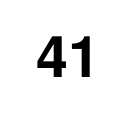
\begin{tikzpicture}
        \node[anchor=north west] at (0,0) {\usefont{OT1}{phv}{b}{n}\huge 41}; % Numéro de l'étape
    \end{tikzpicture}
\end{minipage}%
\hfill

% !! images des pièces 
\begin{minipage}[t]{1\textwidth}
    \begin{tcolorbox}[colback=white, colframe=white!60, boxrule=0.7pt, left=2mm, right=2mm, top=1mm, bottom=1mm]
        \setlength{\extrarowheight}{0pt} % <-- Ajouté pour réduire l'espace vertical
        \begin{tabularx}{\textwidth}{@{}cc@{\hspace{1cm}}cc@{}}
            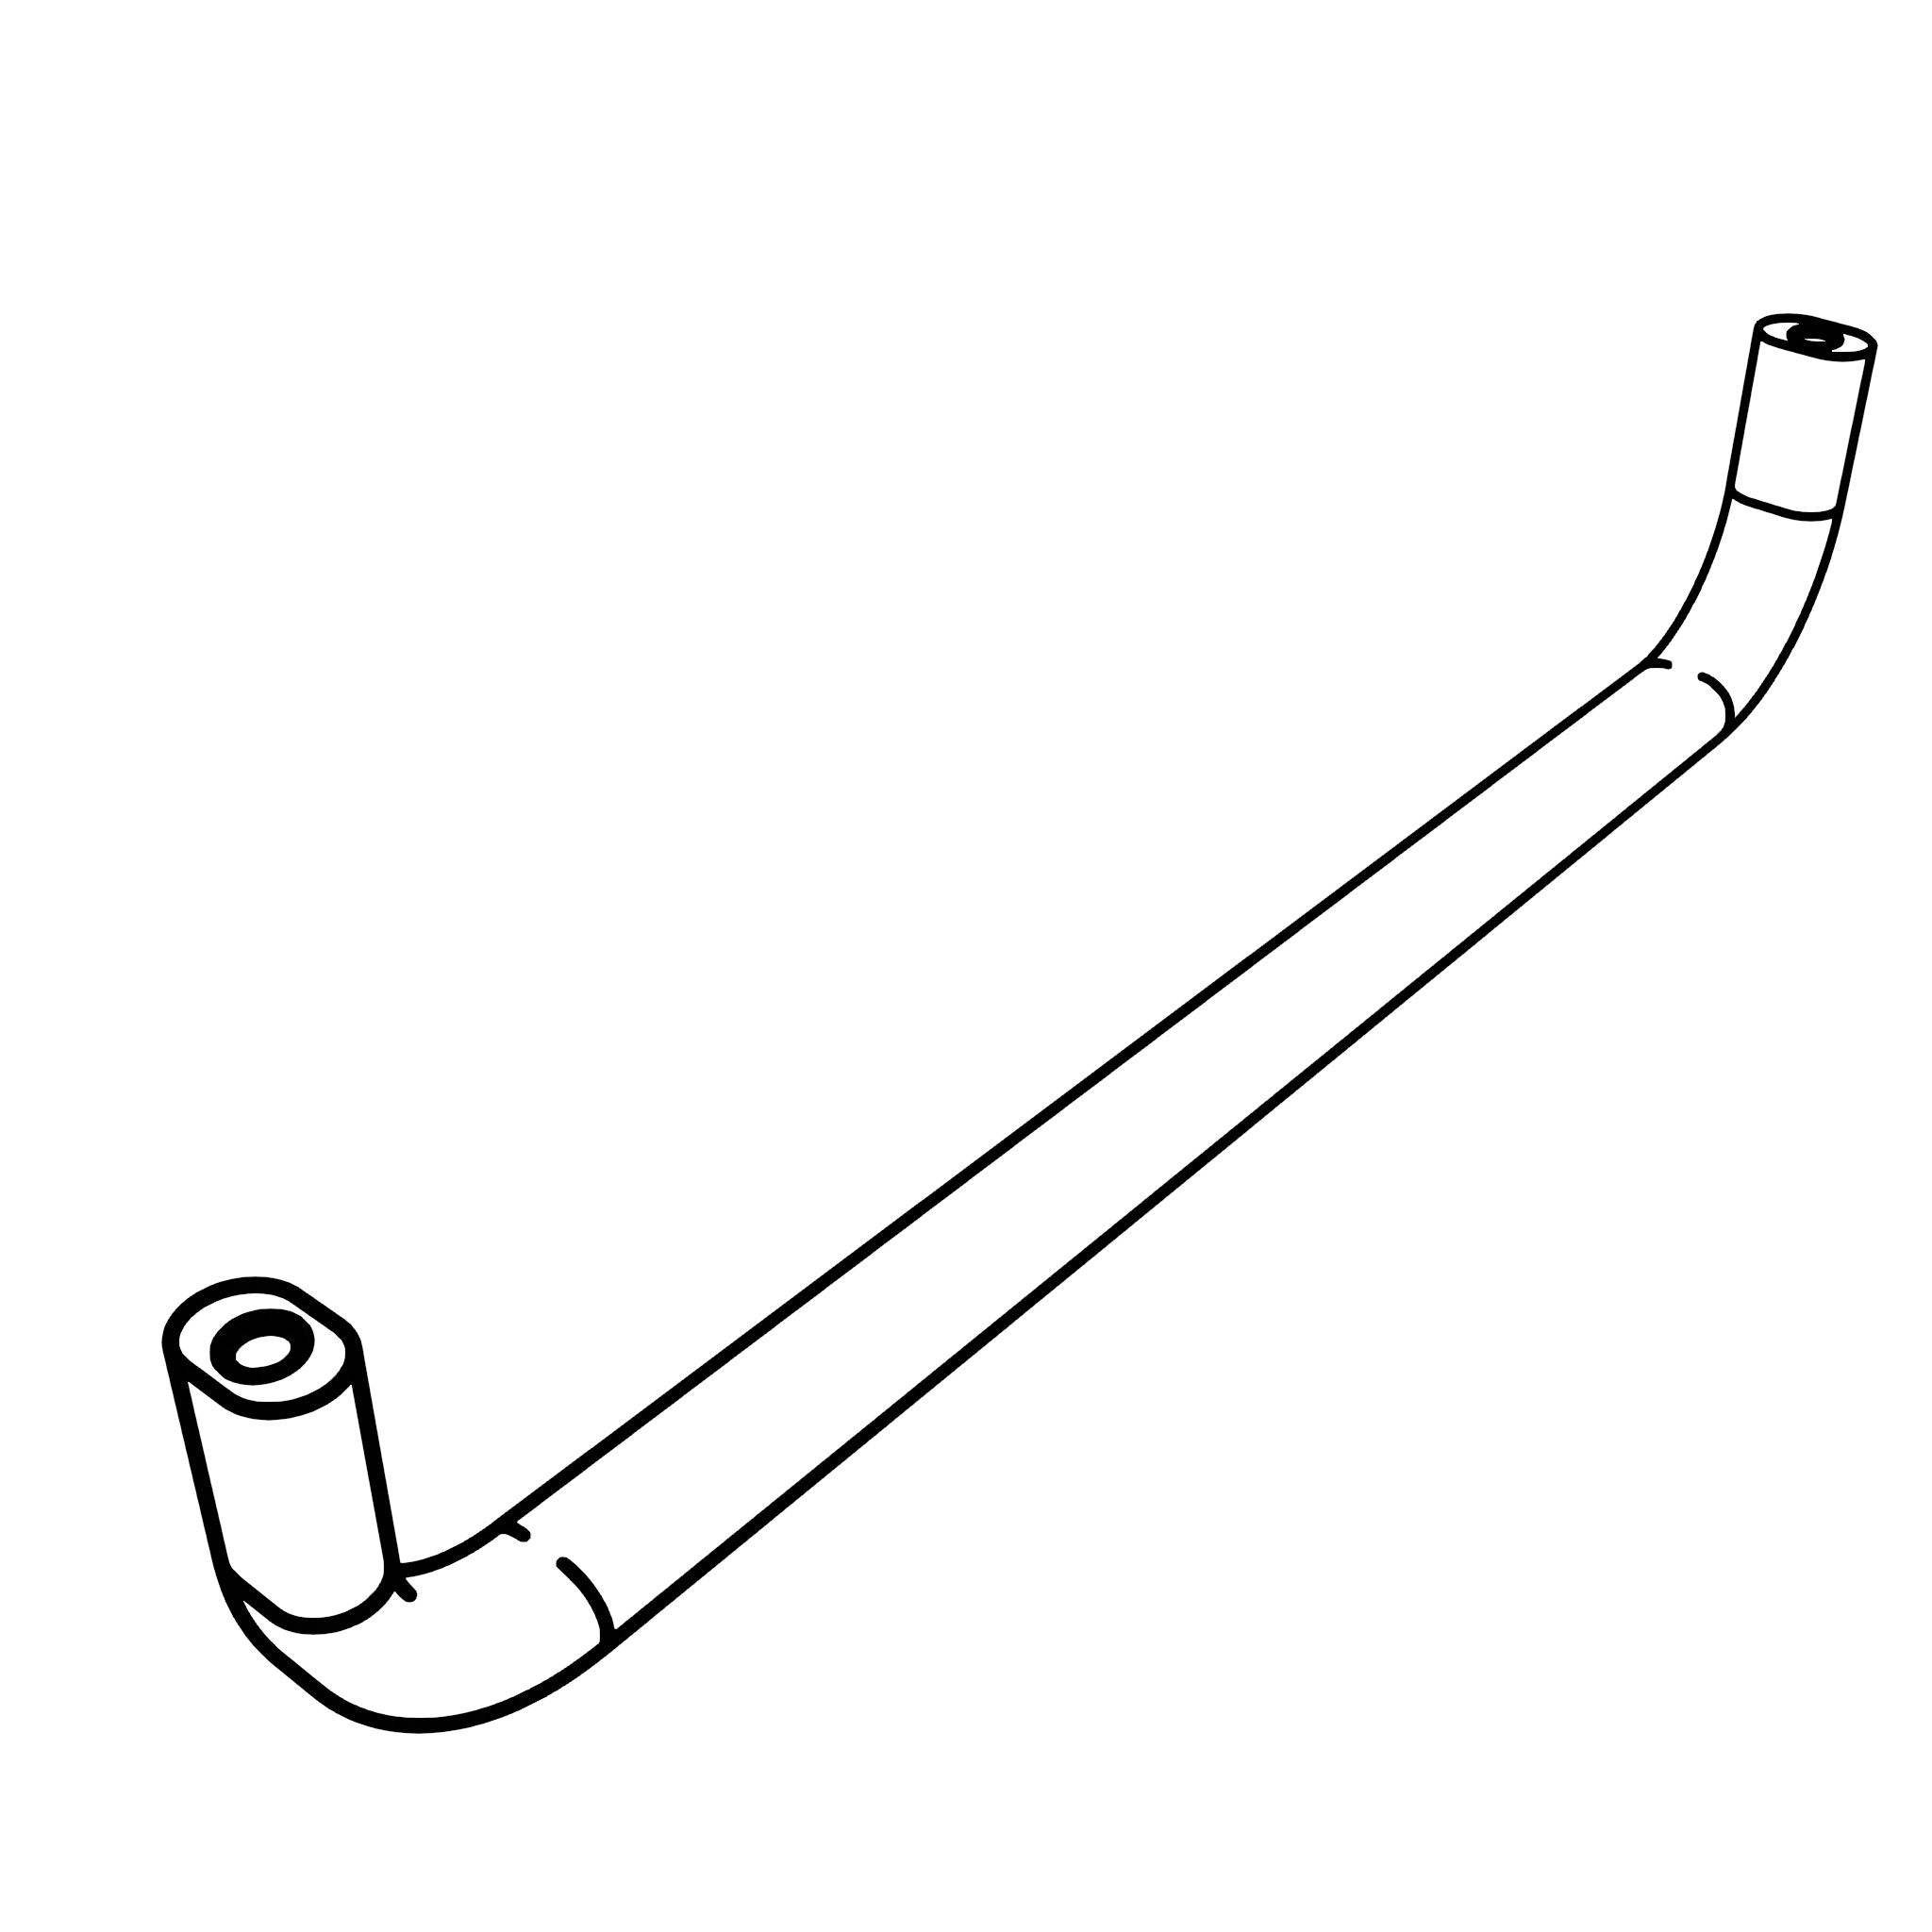
\includegraphics[width=1.5cm]{../images/M04_.png} & \textbf{Handle} $\times$ 1
            & 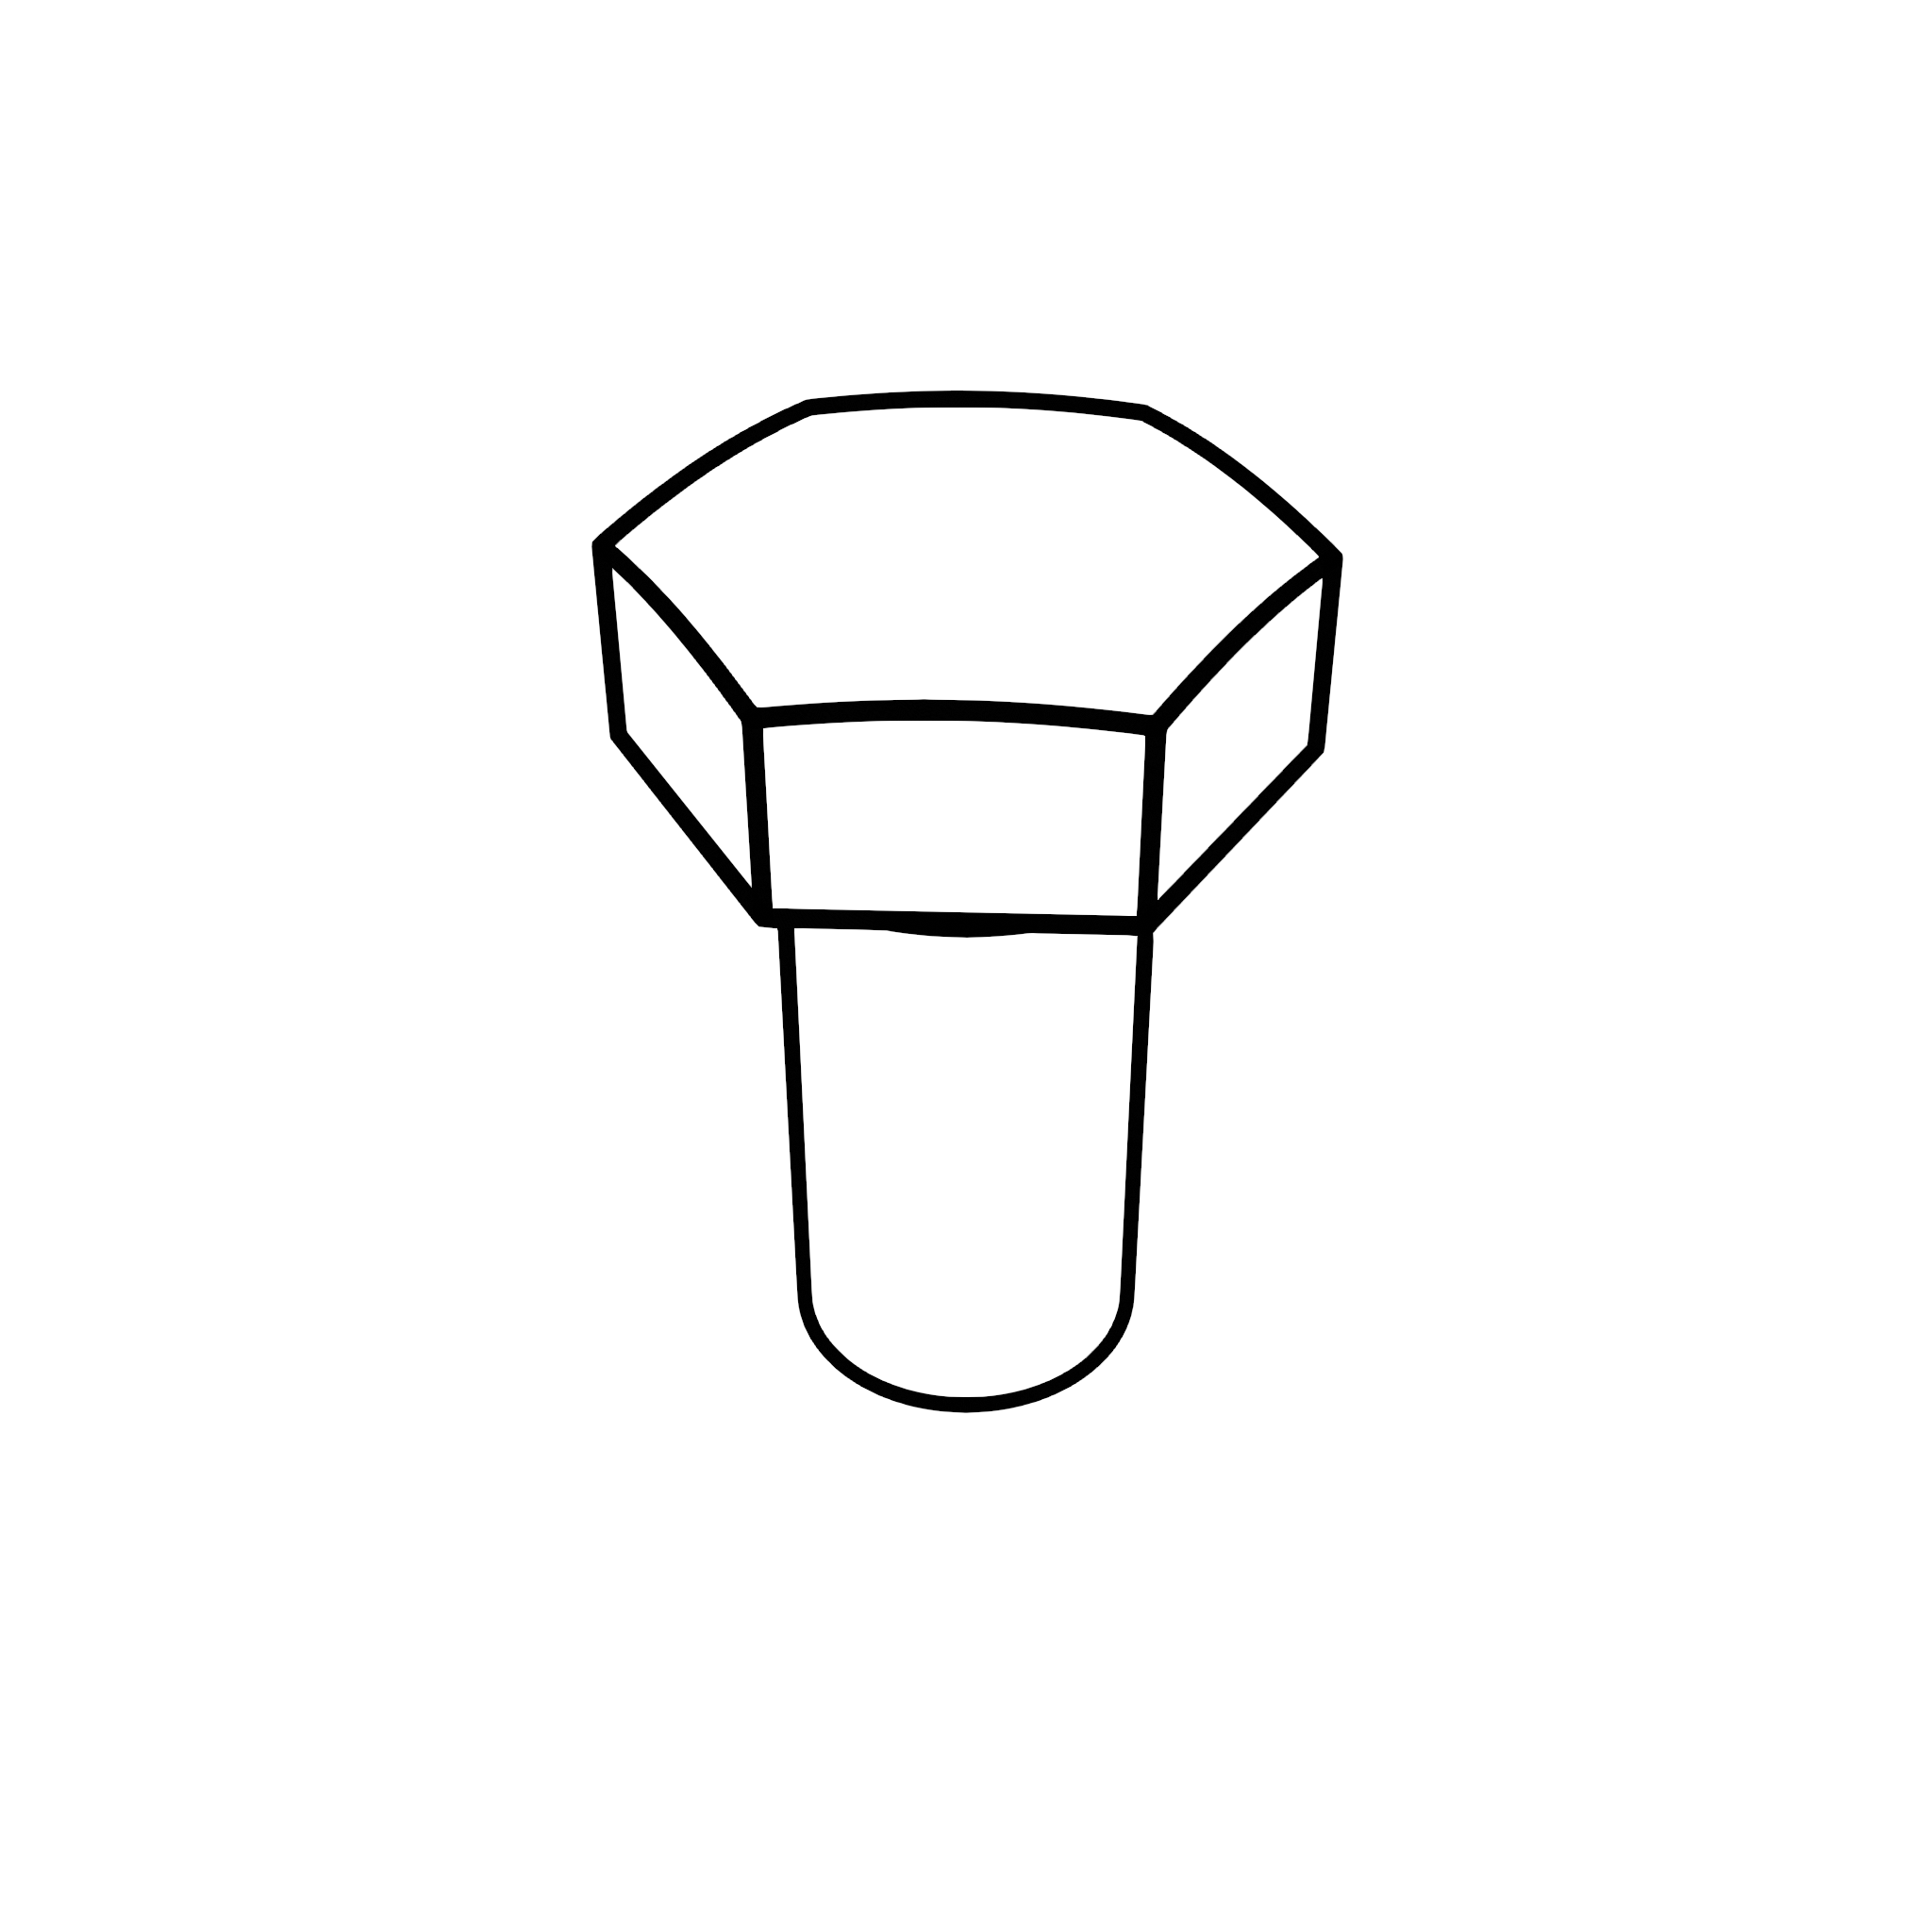
\includegraphics[width=1.5cm]{../images/M05_.png} & \textbf{Hex M5 screw} $\times$\\ 2
            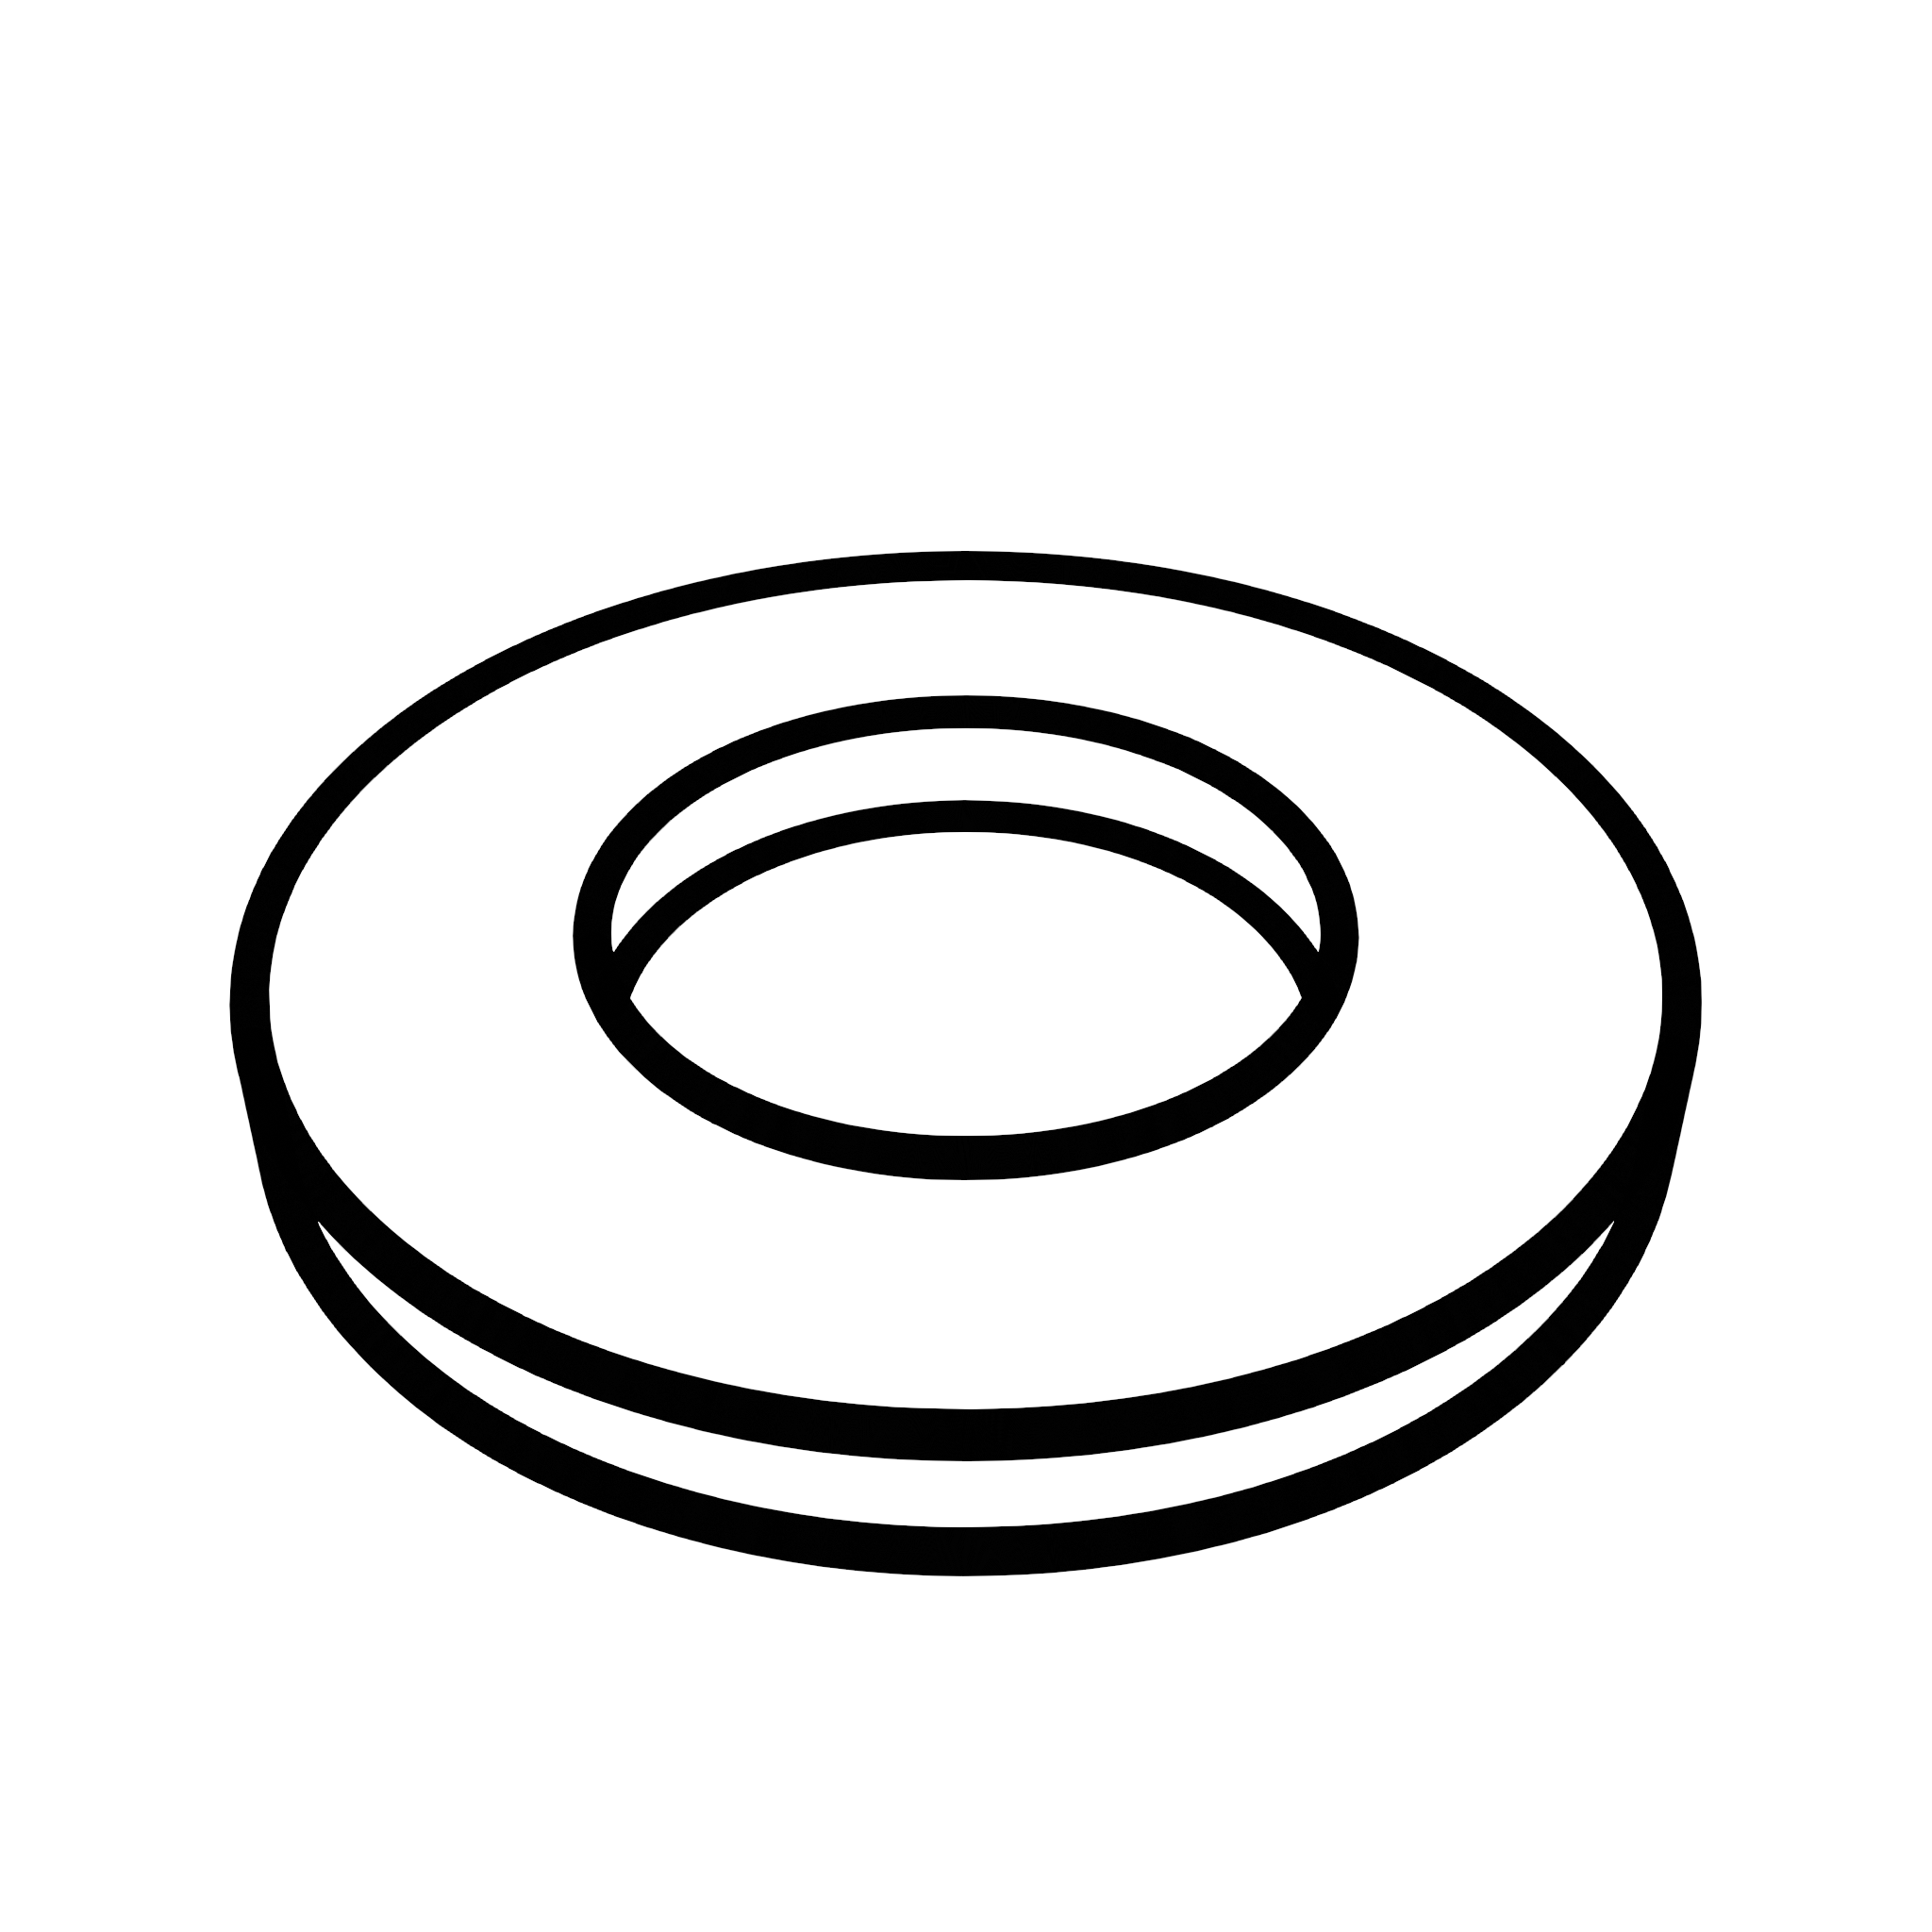
\includegraphics[width=1.5cm]{../images/M06_.png} & \textbf{Spacer} $\times$ 2
           
            %& & \\
        \end{tabularx}
        \setlength{\extrarowheight}{0.5em} % <-- Remet la valeur par défaut si besoin après
    \end{tcolorbox}


    % !! Images des outils centrées à droite
    \vspace{0.05em}
    \noindent
    \begin{flushright}
        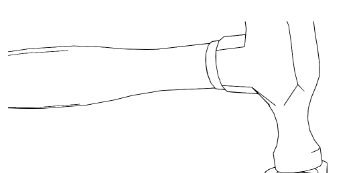
\includegraphics[height=1cm]{../images/tool1.png} \hspace{0.1cm}
        %
\includegraphics[height=1cm]{../images/tool2.png}
    \end{flushright}
\end{minipage}

\vspace{1em}

\begin{center}
    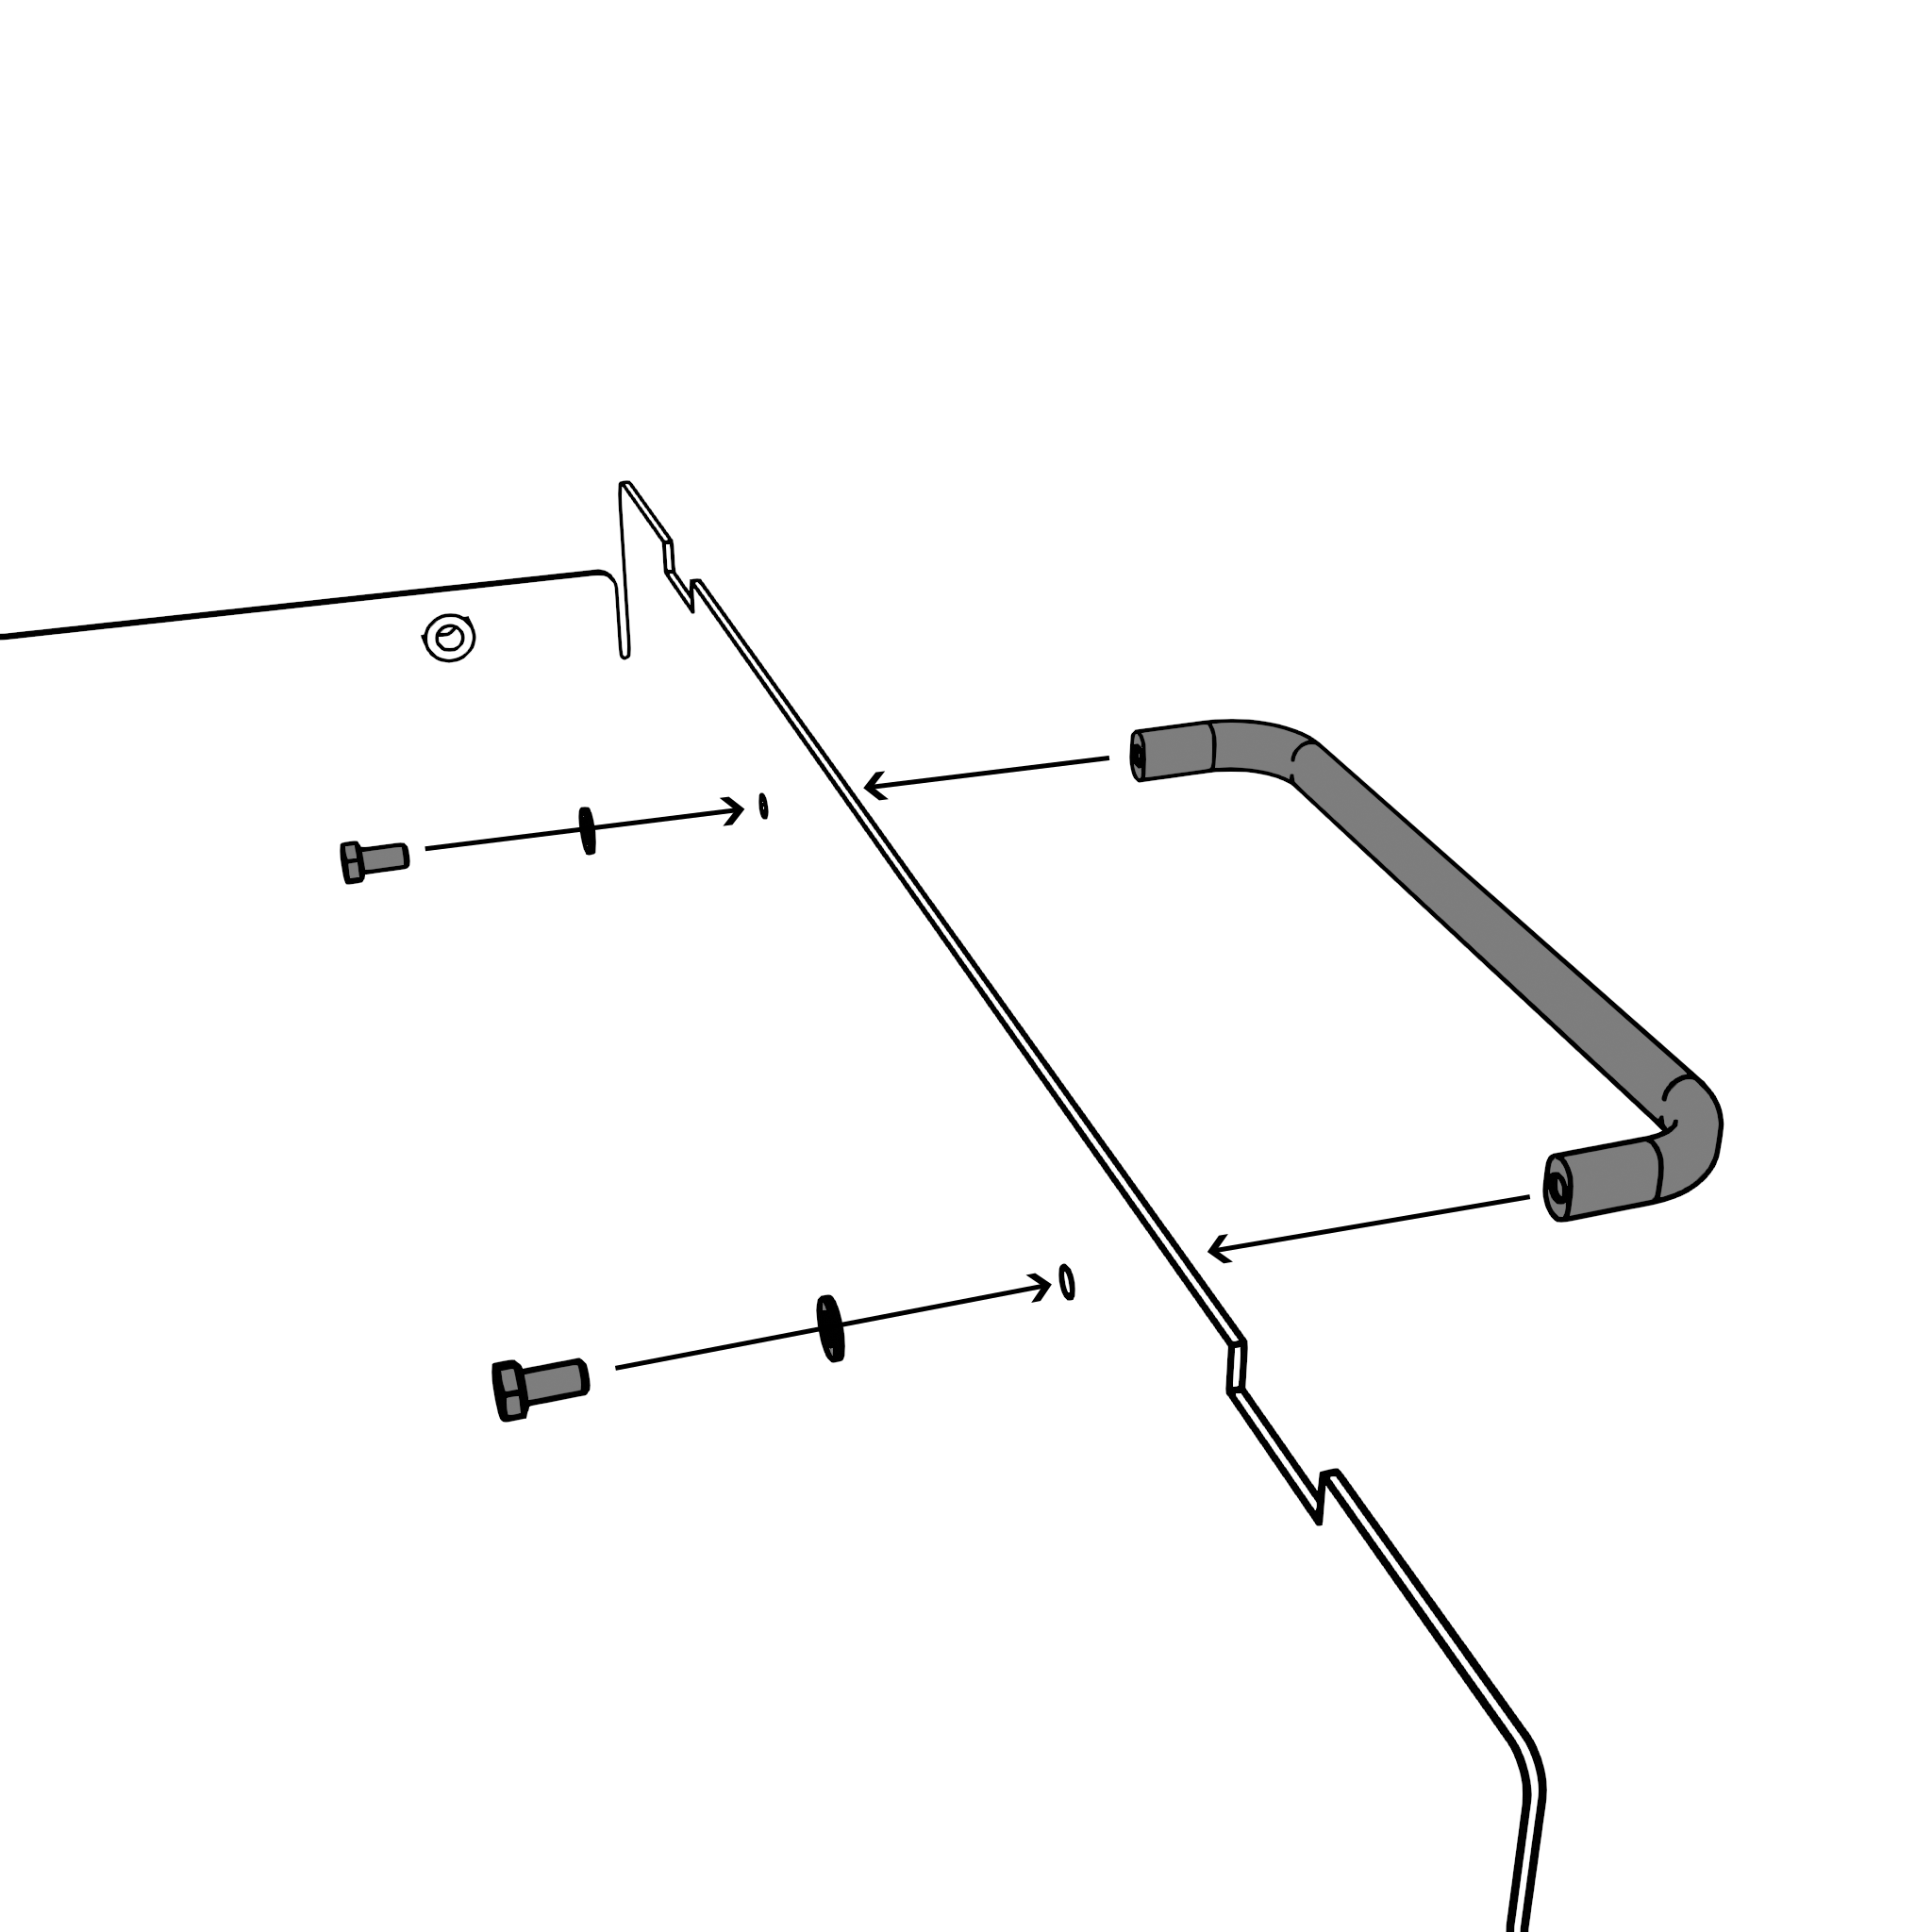
\includegraphics[height=10cm]{../images/_307_.png}
\end{center}

\vspace{0.7em}

%\begin{tcolorbox}[colback=gray!05, colframe=gray!60, boxrule=0.5pt, left=2mm, right=2mm, title=]
%    \begin{enumerate}
%        \item Rassemblez les pièces nécessaires (voir la nomenclature).
%        \item Vérifiez l'allignement entre le pied avant et le plateau du châssis.
%        \item Insérez les vis M5 à travers le pied avant et le plateau du châssis.
%        \item Serrzez les écrous M5 sur les vis.
%        \end{enumerate}
%\end{tcolorbox}


